\section{E\lc{valuation}}

\revision{We use five WCA applications, including FACE, PING PONG, LEGO, POOL,
and IKEA for evaluation~\cite{Chen2017}~\cite{chen2018}. These applications are
selected based on their distinct requirements and characteristics to represent
the variety of WCA apps. IKEA and LEGO assist users step by step to assemble an
IKEA lamp or a LEGO model. While their 2.7-second loose latency bound is less
stringent than other apps, the significance of their instructions is high, as a
user could not proceed without the instruction. On the other hand, users could
still continue their tasks without the instructions from FACE, POOL, and
PING PONG assistants. For POOL and PING PONG, the speed of an instruction is
paramount to its usefulness. For example, any instruction that comes 105ms after
a user action for POOL is no longer of value.}

\begin{figure}
\centering
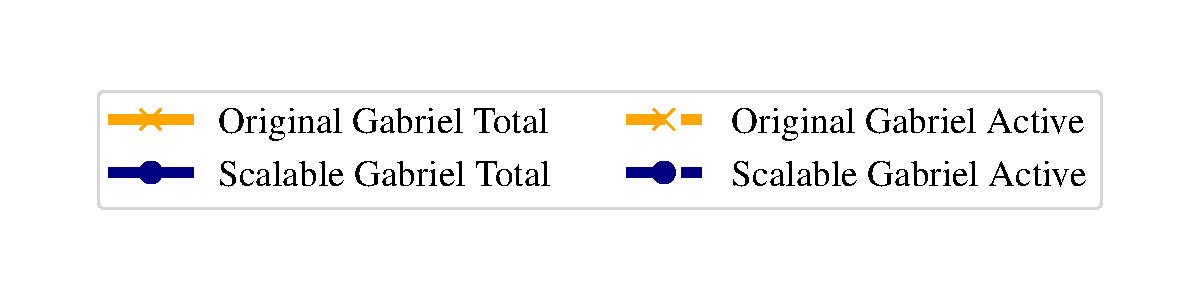
\includegraphics[width=\linewidth, trim=0em 3em 0em 3em, clip]{FIGS/fig-sec6-reduction-legend.pdf}
\begin{minipage}[b]{0.38\linewidth}
\centering
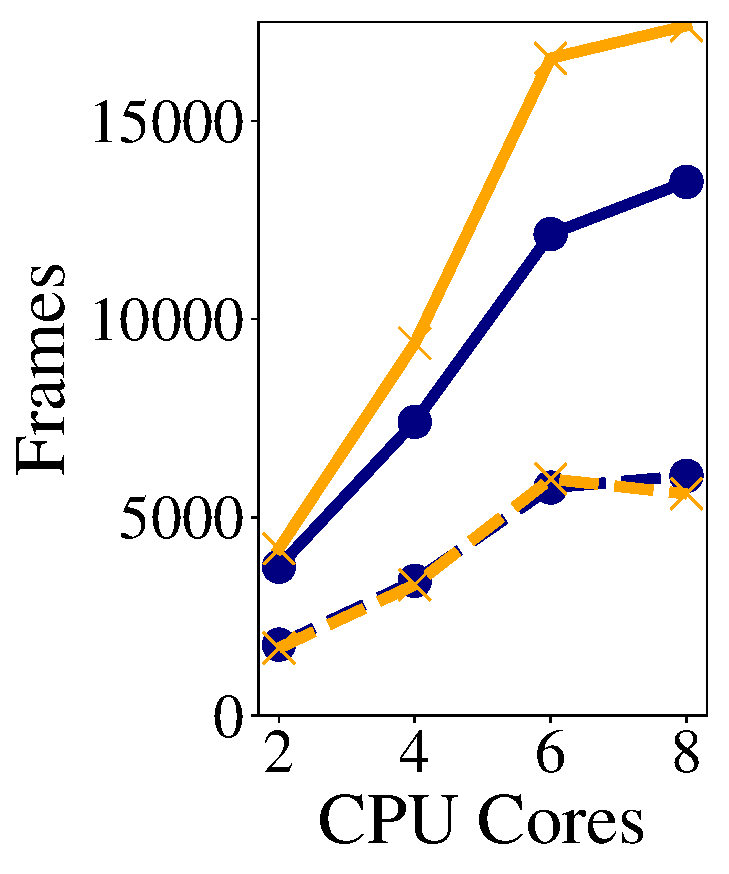
\includegraphics[height=1.3in, trim=0em 1em 0em 0em, clip]{FIGS/fig-sec6-reduction-Pingpong.pdf}\\
{\small (a) PING PONG}
\end{minipage}
\begin{minipage}[b]{0.3\linewidth}
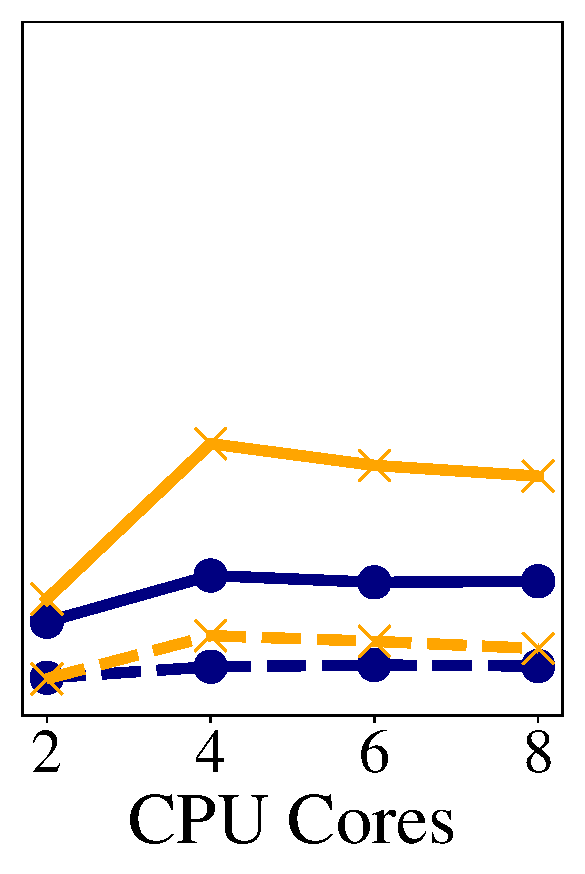
\includegraphics[height=1.3 in, trim=0em 1em 0em 0em, clip]{FIGS/fig-sec6-reduction-Lego.pdf}\\
{\small (b) LEGO}
\end{minipage}
\begin{minipage}[b]{0.3\linewidth}
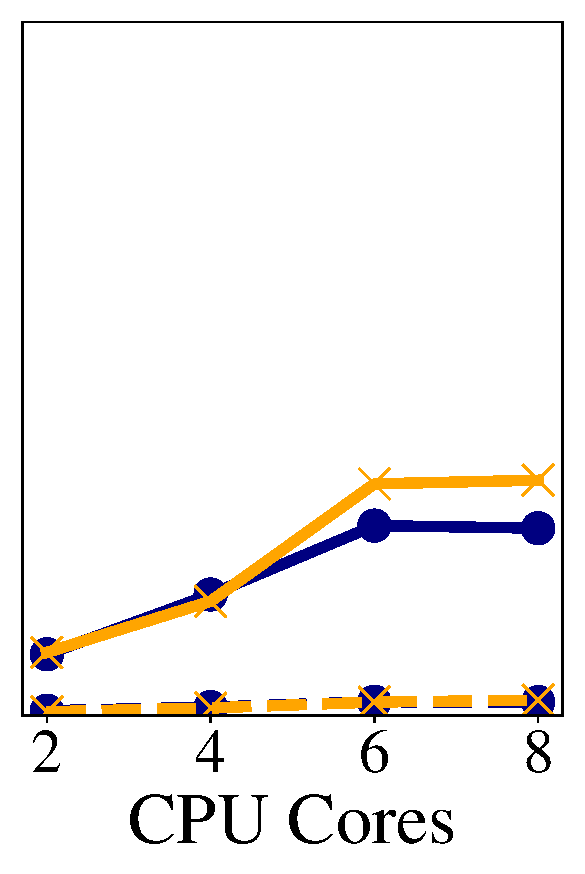
\includegraphics[height=1.3in, trim=0em 1em 0em 0em, clip]{FIGS/fig-sec6-reduction-Pool.pdf}\\
{\small (c) POOL}
\end{minipage}
\caption{\small Effects of Workload Reduction}
\label{figs:workload-reduction}
\end{figure}


\begin{table}
\centering
\begin{tabular}{|c|c||c|c|c|c|c|}
  \hline
  Exp & \multicolumn{6}{|c|}{Number of Clients} \\
  \cline{2-7}
  \#  & Total & FACE & LEGO & POOL & PING & IKEA \\
      &      &   &   &  & PONG &  \\ \hline
  1   & 15  & 3 & 3 & 3 & 3 & 3 \\ \hline
  2   & 20  & 4 & 4 & 4 & 4 & 4 \\ \hline
  3   & 23  & 5 & 5 & 4 & 4 & 5\\ \hline
  4   & 25  & 5 & 5 & 5 & 5 & 5 \\ \hline
  5   & 27  & 5 & 6 & 6 & 5 & 5 \\ \hline
  6  & 30  & 5 & 7 & 6 & 6 & 6 \\ \hline
  7  & 32  & 5 & 7 & 7 & 7 & 6 \\ \hline
  8  & 40  & 8 & 8 & 8 & 8 & 8 \\ \hline
\end{tabular}
\vspace{0.1in}
\caption{\small Resource Allocation Experiments} 
\label{tab:alloc-exps}
\vspace{-0.2in}
\end{table}

\begin{figure}
  \centering
  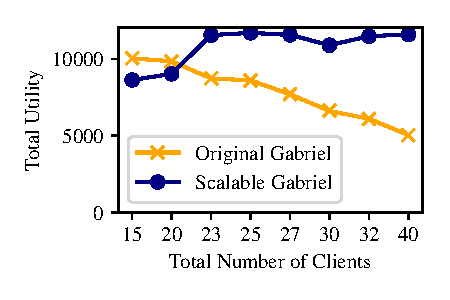
\includegraphics[scale=1.]{FIGS/fig-alloc-max-util.pdf}
  \caption{\small Total Utility with Increasing Contention}
  \label{fig:alloc-max-util}
\end{figure}

\subsection{Effectiveness of Workload Reduction}
We first evaluate the effectiveness of all of the workload reduction
techniques explored in Section~\ref{sec: workload-reduction}. For this
set of experiments, we do not use multiple concurrent applications or
resource allocation. We use four Nexus 6 mobile phones as clients,
connecting to a cloudlet over a Wi-Fi link. We run PING PONG, LEGO,
and POOL applications one at a time with 2, 4, 6, and 8 cores
available on the server. Figure~\ref{figs:workload-reduction} shows
the total number of frames processed with and without workload
reduction. Note that although the offered work is greatly reduced, the
processed frames for active phases of the application have not been
affected. Thus, we confirm that we can significantly reduce cloudlet
load without affecting the critical processing needed by these
applications.


\subsection{Effectiveness of Resource Allocation}

\begin{figure}[t]
  \begin{center}
    
\includegraphics[width=\linewidth]{FIGS/fig-alloc-latency-legend.pdf}
    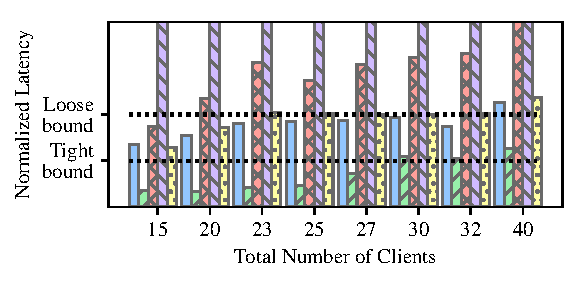
\includegraphics[width=\linewidth]{FIGS/fig-alloc-latency-baseline.pdf}
    {\small (a) Original Gabriel}
    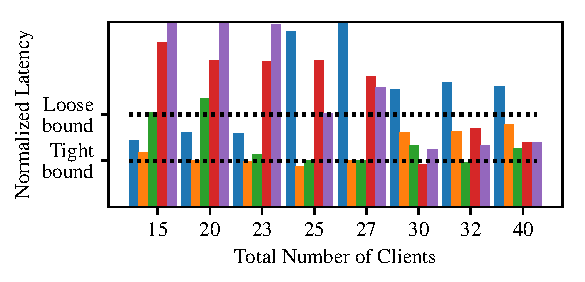
\includegraphics[width=\linewidth]{FIGS/fig-alloc-latency-cpushares.pdf}
    {\small (b) Scalable Gabriel}
  \end{center}
\begin{captiontext}
The normalization is  by per-application tight and loose bounds~\cite{Chen2017}
\end{captiontext}
\vspace{-0.1in}
  \caption{\small Normalized 90\%-tile Response Latency}
  \label{fig:alloc-latency}
\end{figure}

\begin{figure}[t]
  \begin{center}
    
\includegraphics[width=\linewidth]{FIGS/fig-alloc-latency-legend.pdf}
    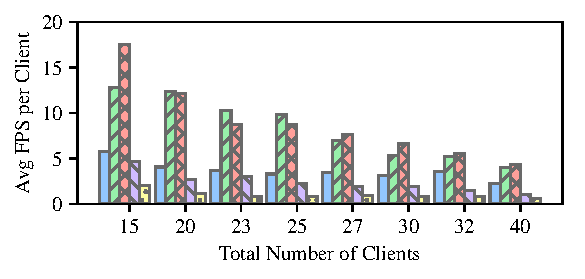
\includegraphics[width=\linewidth]{FIGS/fig-alloc-fps-baseline.pdf}
    {\small (a) Original Gabriel}
    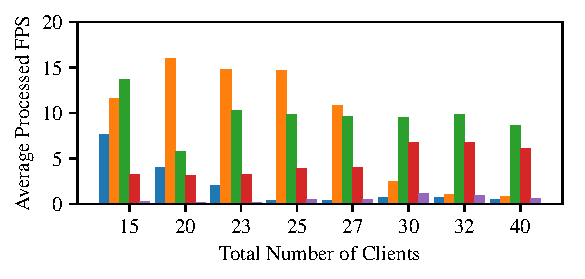
\includegraphics[width=\linewidth]{FIGS/fig-alloc-fps-cpushares.pdf}
    {\small (b) Scalable Gabriel}
  \end{center}
\vspace{-0.1in}
  \caption{\small Average Processed Frames Per Second Per Client}
  \label{fig:alloc-fps}
\vspace{-0.1in}
\end{figure}

We next evaluate resource allocation on a server machine with 2
Intel{\textregistered} Xeon{\textregistered} E5-2699 v3 processors, totaling 36
physical cores running at 2.3 Ghz (turbo boost disabled) and 128 GB memory. We
dedicate 8 physical cores (16 Intel{\textregistered} hyper threads) and 16 GB memory as cloudlet
resources using cgroup. We run 8 experiments with increasing numbers of clients
across four concurrent applications with a total of 15 to 40 clients. The
breakdown of the number of clients used for each experiment is given in
Table~\ref{tab:alloc-exps}. We use offline generated application profiles
discussed in Section~\ref{sec: resource-allocation} to optimize for total system
utility. Figure~\ref{fig:alloc-max-util} shows how the system-wide total utility
changes as we add more clients to the workload, under the original Gabriel
approach and the scalable Gabriel approach. We see that original Gabriel's total
utility drops more than 40\% as contention increases, since every client
contends for resources in an uncontrolled fashion.  All applications suffer, but
the effects of increasing latencies are vastly different among different
applications. In contrast, scalable Gabriel maintains a high level of
system-wide utility by differentially allocating resources to different
applications based on their sensitivity captured in the utility profiles.


Figure~\ref{fig:alloc-latency} and Figure~\ref{fig:alloc-fps} provide insights
into how scalable Gabriel strikes the balance. Latencies are better controlled
as resources are dedicated to applications with high utility, and more clients
are kept within their latency bounds. Of course, with higher contention, fewer
frames per second can be processed for each client. Original Gabriel degrades
applications in an undifferentiated fashion. Scalable Gabriel, in contrast,
tries to maintain higher throughput for some applications at the expense of the
others, e.g. LEGO up to 25 clients.


\subsection{Effects on Guidance Latency}

\begin{figure}
	\begin{center}
		
\includegraphics[width=\linewidth]{FIGS/fig-alloc-latency-legend.pdf}
								
		\begin{tabular}{c@{}c}
			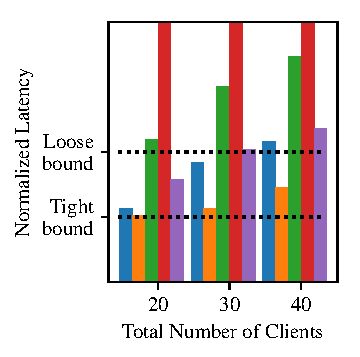
\includegraphics[width=.5\linewidth]{FIGS/fig-eval-latency-baseline.pdf}
			            & 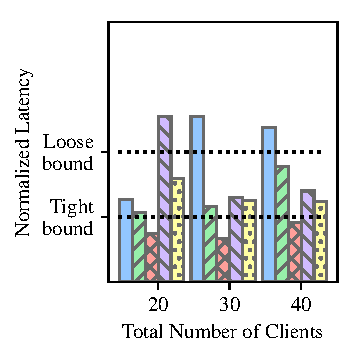
\includegraphics[width=.5\linewidth]{FIGS/fig-eval-latency-cpushares.pdf} \\
			{\small (a) Original  Gabriel} & {\small (b) Scalable Gabriel}                                                    
		\end{tabular}
	\end{center}

\begin{captiontext}
The normalization is by per-application tight and loose bounds~\cite{Chen2017}
\end{captiontext}
\vspace{-0.1in}
	\caption{\small Normalized 90\%-tile Response Latency}
	\label{fig:frame-latency}
\end{figure}

\begin{figure}
	\begin{center}
		
\includegraphics[width=\linewidth]{FIGS/fig-alloc-latency-legend.pdf}
		\begin{tabular}{c@{}c}
			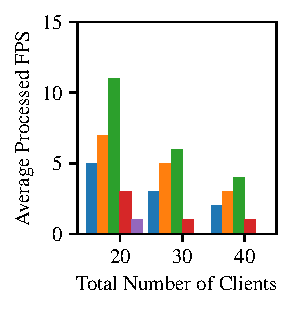
\includegraphics[width=.5\linewidth]{FIGS/fig-eval-fps-baseline.pdf}
			            & 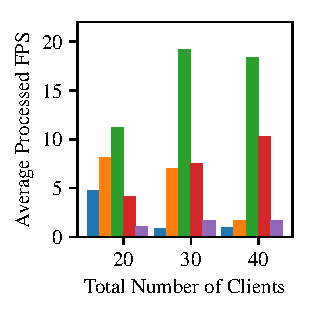
\includegraphics[width=.5\linewidth]{FIGS/fig-eval-fps-cpushares.pdf} \\
			{\small (a) Original Gabriel} & {\small (b) Scalable Gabriel}                                                
		\end{tabular}
	\end{center}
	\caption{\small Processed Frames Per Second Per Application}
	\label{fig:frame-fps}
\end{figure}

\begin{figure}
\centering
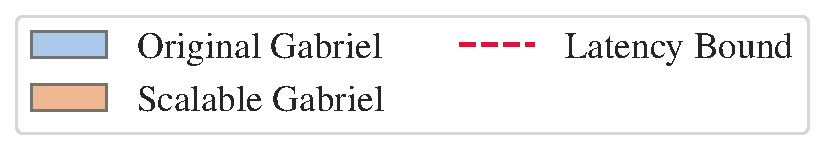
\includegraphics[width=0.7\linewidth, trim=0em 0em 0em 0em, clip]{FIGS/fig-sec6-latency-legend.pdf} \\
\centering
\begin{turn}{90}{\hspace{0.6in}\small (a) FACE}\end{turn}\hspace{0.2in}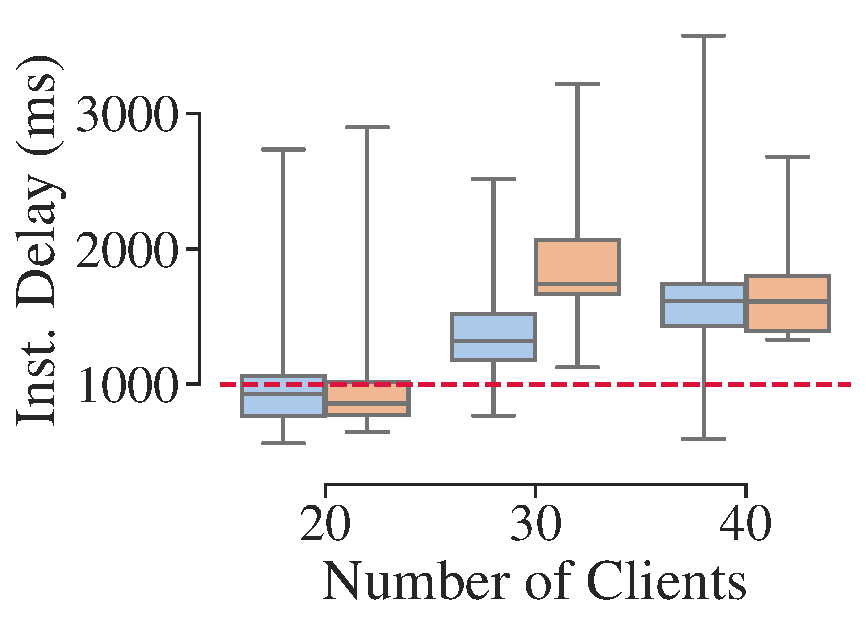
\includegraphics[width=2.1in, trim=0em 0em 0em 0em, clip]{FIGS/fig-sec6-latency-face.pdf}\\[0.08in]
\begin{turn}{90}{\hspace{0.6in}\small (b) LEGO}\end{turn}\hspace{0.2in}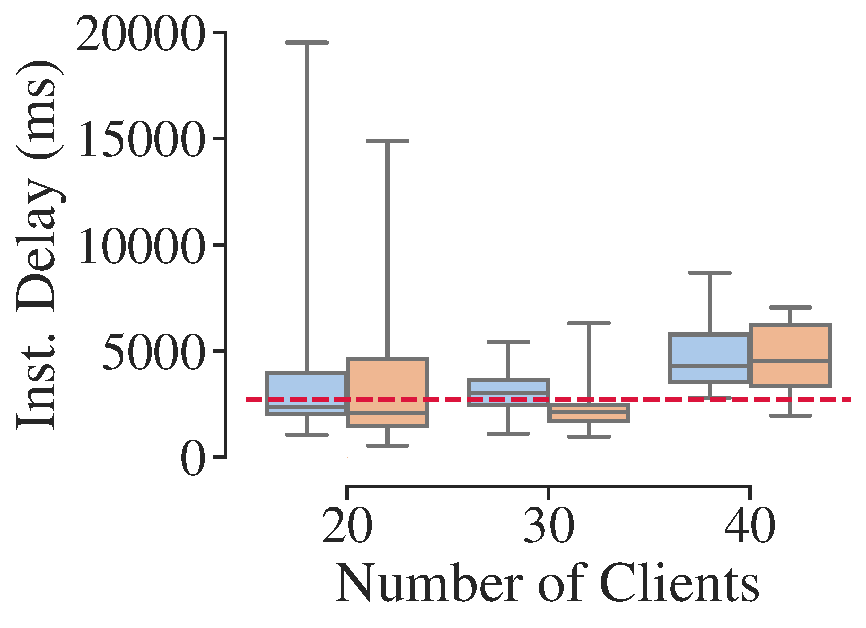
\includegraphics[width=2.1in, trim=0em 0em 0em 0em, clip]{FIGS/fig-sec6-latency-lego.pdf}\\[0.08in]
\begin{turn}{90}{\hspace{0.6in}\small (c) PING PONG}\end{turn}\hspace{0.2in}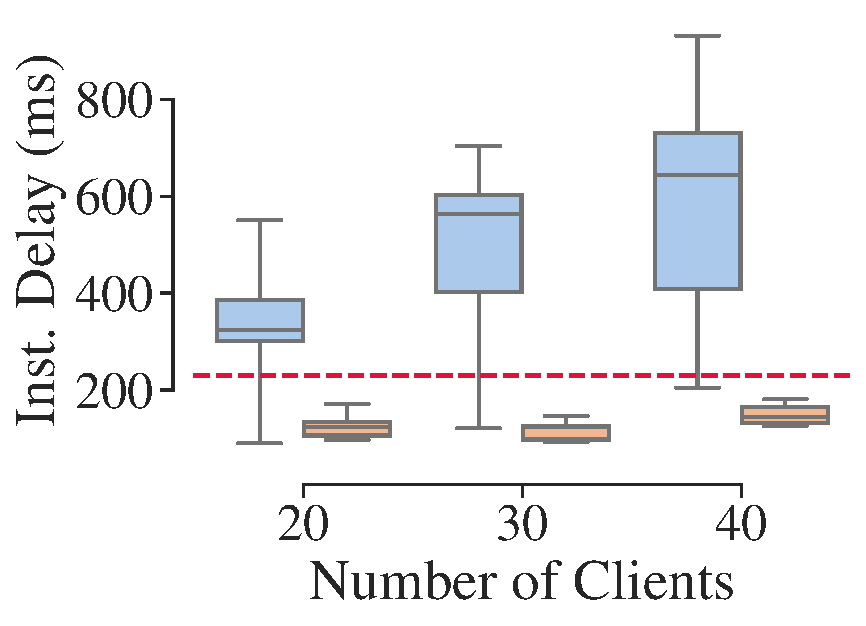
\includegraphics[width=2.1in, trim=0em 0em 0em 0em, clip]{FIGS/fig-sec6-latency-pingpong.pdf}\\[0.08in]
\begin{turn}{90}{\hspace{0.6in}\small (d) POOL}\end{turn}\hspace{0.2in}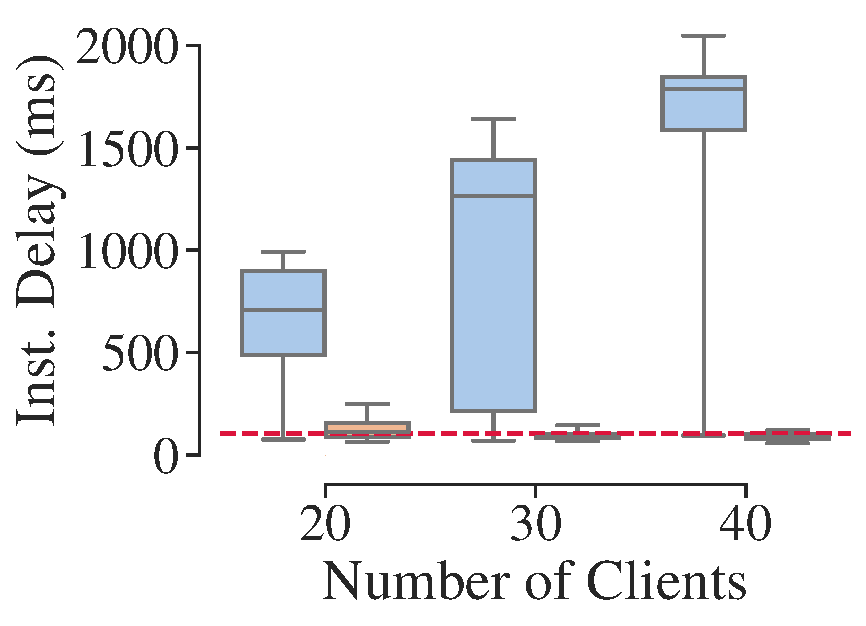
\includegraphics[width=2.1in, trim=0em 0em 0em 0em, clip]{FIGS/fig-sec6-latency-pool.pdf}\\[0.08in]
\begin{turn}{90}{\hspace{0.6in}\small (e) IKEA}\end{turn}\hspace{0.2in}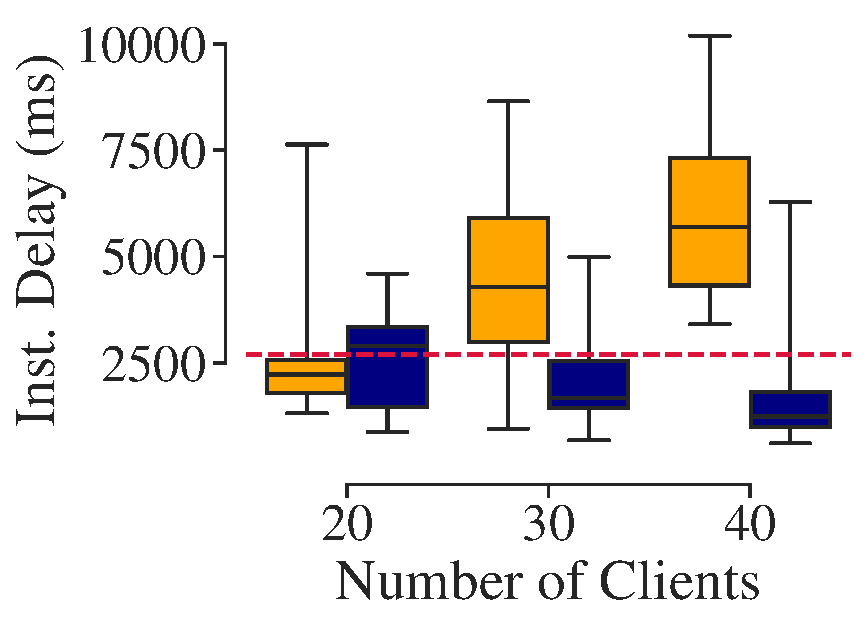
\includegraphics[width=2.1in, trim=0em 0em 0em 0em, clip]{FIGS/fig-sec6-latency-ikea.pdf}
  \vspace{-0.1in}
\caption{\small Guidance Latency}
\label{figs:inst-delay}
\end{figure}
		
We next evaluate the combined effects of workload reduction and
resource allocation in our system. We emulate many users running
multiple applications simultaneously. All users share the same
cloudlet with 8 physical cores and 16 GB memory. We conduct three experiments,
with 20 (4 clients per app), 30 (6 clients per app), and 40 (8 clients
per app) clients. Each client loops through pre-recorded video traces
with random starting points.  Figure~\ref{fig:frame-latency} and
Fig~\ref{fig:frame-fps} show per client frame latency and FPS
achieved. The first thing to notice is that concurrently utilizing
both sets of techniques does not cause conflicts. In fact, they appear
to be complementary and latencies remain in better control than using
resource allocation alone.

\begin{figure}
	\begin{center}
		
\includegraphics[width=\linewidth]{FIGS/fig-alloc-latency-legend.pdf}
		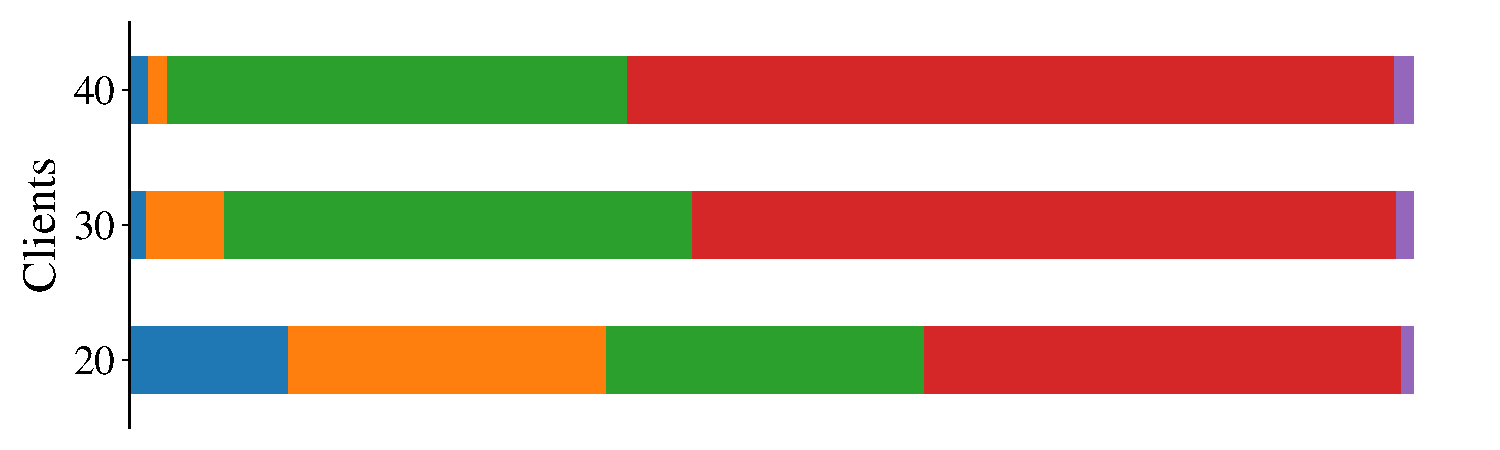
\includegraphics[width=\linewidth]{FIGS/fig-sec6-latency-allocation.pdf}
	\end{center}
\vspace{-0.1in}
	\caption{\small Fraction of Cloudlet Processing Allocated}
	\label{figs:resource-allocated}
\end{figure}

The previous plots consider per request latencies. The ultimate goal
of our work is to maintain user experience as much as possible and
degrade it gracefully when overloaded. For WCA applications, the key
measure of user experience is guidance latency, the time between the
occurrence of an event and the delivery of corresponding guidance.
Figure~\ref{figs:inst-delay} shows boxplots of per-application
guidance latency for the concurrent application experiments above. The
red line denotes the application-required loose bound. It is clear
that our methods control latency significantly better than the
baseline. Scalable Gabriel is able to serve at least 3x number of clients
when moderately loaded while continuing to serve half of the clients
when severely loaded. In these experiments, the utility is maximized
at the expense of the FACE application, which provides the least
utility per resource consumed. At the highest number of clients, scalable
Gabriel sacrifices the LEGO application to maintain the quality of service for
the other two. This differentiated allocation is reflected in
Figure~\ref{figs:resource-allocated}. In contrast, with original Gabriel,
none of the applications are able to regularly meet deadlines.









